\documentclass[11pt,a4paper]{article}

% --- Paquetes de Estilo y Formato ---
\usepackage[utf8]{inputenc}
\usepackage[spanish,es-tabla]{babel}
\usepackage[T1]{fontenc}
\usepackage{geometry}
\geometry{top=3cm, bottom=3cm, left=3cm, right=2.5cm}
\usepackage{tabularx}
\usepackage{titlesec}
\usepackage{fancyhdr}
\usepackage{lastpage}
\usepackage{hyperref}
\usepackage{enumitem}
\usepackage{graphicx}
\usepackage{tikz}
\usepackage{float}
\usepackage[table, xcdraw]{xcolor}

% --- Definición de Colores Corporativos ArthroDesign ---
\definecolor{ArthroNavy}{HTML}{0F172A}
\definecolor{ArthroTeal}{HTML}{0D9488}
\definecolor{ArthroGray}{HTML}{64748B}

% --- Configuración de Párrafo ---
\setlength{\parskip}{0.5em}
\setlength{\parindent}{1.5em}

% --- Estilo de Títulos con Identidad Corporativa ---
\titleformat{\section}
  {\color{ArthroNavy}\Large\bfseries}
  {\thesection.}
  {0.5em}
  {}
  [{\color{ArthroTeal}\titlerule[1.5pt]}]

\titleformat{\subsection}
  {\color{ArthroNavy}\large\bfseries}
  {\thesubsection.}
  {0.5em}
  {}
  [{\color{ArthroTeal}\titlerule[1pt]}]

\titleformat{\subsubsection}
  {\color{ArthroNavy}\large\bfseries}
  {\thesubsubsection.}
  {0.5em}
  {}

% --- Viñetas en color Turquesa ---
\renewcommand{\labelitemi}{\color{ArthroTeal}\textbullet}
\renewcommand{\labelitemii}{\color{ArthroTeal}\circ}

% --- Configuración de Enlaces ---
\hypersetup{colorlinks=true, linkcolor=ArthroNavy, urlcolor=ArthroTeal}

% --- CONFIGURACIÓN DE ENCABEZADO Y PIE CORPORATIVO (Anexo VIII) ---
\pagestyle{fancy}
\fancyhf{}

% Línea superior de color turquesa (Grosor 2pt)
\renewcommand{\headrule}{\hbox to\headwidth{\color{ArthroTeal}\leaders\hrule height 2pt\hfill}}

% Información de Encabezado
\fancyhead[L]{\small \textbf{\color{ArthroNavy}Adaptador ergonómico - PR-PIB-GIS26-09}}
\fancyhead[R]{\small \textbf{\color{ArthroNavy}Anexo XII: Etiqueta e instrucciones}}

% Información de Pie de Página
\fancyfoot[L]{\small \color{ArthroGray}ArthroDesign Solutions S.L.}
\fancyfoot[C]{\small \color{ArthroGray}\today}
\fancyfoot[R]{\small \textbf{\color{ArthroNavy}Pág. \thepage \ de \pageref{LastPage}}}

\setlength{\headheight}{15pt}
\renewcommand{\footrulewidth}{0.4pt}

\begin{document}

% ======================================================
% PÁGINA 1: PORTADA
% ======================================================
\begin{titlepage}
    % --- Elementos Geométricos de Identidad (Cabecera y Pie) ---
    \begin{tikzpicture}[remember picture,overlay]
        % Franja superior
        \fill[ArthroNavy] (current page.north west) rectangle ([yshift=-4.5cm]current page.north east);
        \fill[ArthroTeal] ([yshift=-4.5cm]current page.north west) rectangle ([yshift=-4.7cm]current page.north east);
        
        % Franja inferior
        \fill[ArthroNavy] (current page.south west) rectangle ([yshift=2.5cm]current page.south east);
        \fill[ArthroTeal] ([yshift=2.5cm]current page.south west) rectangle ([yshift=2.7cm]current page.south east);
    \end{tikzpicture}

    \centering % Todo centrado a partir de aquí

    % --- LOGO (Sobre la franja azul) ---
    \vspace*{-2cm}
    
\includegraphics[width=6.5cm]{logo_definitivo.png} \\
    \vspace{2cm}

    % --- BLOQUE DE TÍTULO PRINCIPAL ---
    {\color{ArthroGray}\Huge \textbf{ANEXO XII}} \\
    \vspace{0.5cm}
    {\color{ArthroNavy}\Huge \textbf{ETIQUETA E INSTRUCCIONES}} \\
    \vspace{0.3cm}
    {\color{ArthroTeal}\rule{12cm}{2pt}} \\
    \vspace{1cm}
    {\Large \textbf{TÍTULO DEL PROYECTO:}} \\
    \vspace{0.3cm}
    {\Huge \bfseries Diseño de un adaptador ergonómico universal para la optimización de la pulsación manual en inhaladores de dosis medida (MDI)} \\
    \vspace{1.5cm}

    % --- BLOQUE DE IDENTIFICACIÓN TÉCNICA ---
    \begin{minipage}{0.8\textwidth}
        \centering
        \textbf{CÓDIGO DE IDENTIFICACIÓN:} \\
        {\large \texttt{PR-PIB-GIS26-09}} \\[0.8cm]
        
        \textbf{EMPRESA DESARROLLADORA:} \\
        {ArthroDesign Solutions S.L.}
    \end{minipage}

    \vspace{1.5cm}

    % --- BLOQUE DE PROYECTISTAS ---
    \textbf{PROYECTISTAS (Equipo de ArthroDesign Solutions S.L.):} \\
    \vspace{0.3cm}
    \small
    \renewcommand{\arraystretch}{1.3}
    \begin{tabular}{l l}
        \textbf{D. Sergio Carmona Muñoz} & Colegiado Nº 06424 (DNI: 26291930D) \\
        \textbf{D. Juan Gabriel Navarro Valdivielso} & Colegiado Nº 06425 (DNI: 77666662D) \\
        \textbf{D. Antonio Sánchez Doña} & Colegiado Nº 06423 (DNI: 79380534J) \\
        \textbf{D. Iván de la Torre Segato} & Colegiado Nº 06421 (DNI: 79383630G) \\
    \end{tabular}
    
    \vfill

    % --- PIE DE PORTADA ---
    {\color{white} ArthroDesign Solutions S.L. \quad | \quad \today}
    \vspace{-1.75cm} 
\end{titlepage}

% AÑADE ESTA LÍNEA AQUÍ PARA QUE LA SIGUIENTE PÁGINA SEA LA 2:
\setcounter{page}{2}

% ======================================================
% HOJA EN BLANCO CON MARCA DE AGUA
% ======================================================
\newpage
\pagestyle{fancy}

\begin{tikzpicture}[remember picture, overlay]
    \node[opacity=0.1] at (current page.center) {
\includegraphics[width=12cm]{logo_definitivo.png}};
\end{tikzpicture}

% Empujamos el texto hacia la parte inferior del folio
\vspace*{8.5cm} 
\begin{center}
    \textit{Esta hoja ha sido dejada deliberadamente en blanco.}
\end{center}
\vfill
\newpage

% ======================================================
% PÁGINA: ÍNDICE AUTOMÁTICO (CON ENCABEZADO)
% ======================================================
\markboth{Índice}{Índice}
\tableofcontents
\thispagestyle{fancy} % Fuerza el estilo fancy en esta página
\newpage

% ======================================================
% HOJA EN BLANCO CON MARCA DE AGUA
% ======================================================
\newpage
\pagestyle{fancy}

\begin{tikzpicture}[remember picture, overlay]
    \node[opacity=0.1] at (current page.center) {
\includegraphics[width=12cm]{logo_definitivo.png}};
\end{tikzpicture}

% Empujamos el texto hacia la parte inferior del folio
\vspace*{8.5cm} 
\begin{center}
    \textit{Esta hoja ha sido dejada deliberadamente en blanco.}
\end{center}
\vfill
\newpage

% ======================================================
% CONTENIDO DEL ANEXO XII
% ======================================================


\section{ETIQUETADO DEL PRODUCTO}


\subsection{Diseño propuesto de la etiqueta exterior}

La etiqueta exterior se plantea como una etiqueta rectangular, situada en la cara visible del embalaje individual. Debe permitir identificar rápidamente el producto en farmacia, ortopedia, centro sanitario o domicilio del usuario.

\begin{figure}[H]
\centering
\resizebox{\textwidth}{!}{%
\begin{tikzpicture}[x=1cm,y=1cm,font=\sffamily]

% ======================================================
% FONDO GENERAL
% ======================================================
\fill[white] (0,0) rectangle (18,9);

% Marco exterior
\draw[ArthroTeal!45, line width=1.4pt, rounded corners=10pt] (0.25,0.25) rectangle (17.75,8.75);

% Fondo interior suave
\fill[ArthroTeal!7, rounded corners=9pt] (0.35,0.35) rectangle (17.65,8.65);
\fill[white, rounded corners=8pt] (0.55,0.55) rectangle (17.45,8.45);

% Detalles decorativos suaves
\fill[ArthroTeal!25] (0.85,8.05) -- (1.85,8.05) -- (2.15,7.25) -- (0.85,7.55) -- cycle;
\fill[ArthroNavy!18] (15.85,8.05) -- (16.95,8.05) -- (16.95,7.35) -- (15.75,7.1) -- cycle;
\fill[ArthroNavy!12] (0.85,1.0) -- (2.1,1.0) -- (1.7,0.45) -- (0.65,0.6) -- cycle;

% ======================================================
% COLUMNA IZQUIERDA: LOGOS + PROTOTIPO
% ======================================================

% Logo icono
\node[anchor=north west] at (3.05,8.05)
{
\includegraphics[width=1.05cm]{ANEXOS/LogoEmpresa.jpeg}};

% Logo escrito
\node[anchor=north west] at (1.55,7.15)
{
\includegraphics[width=4.15cm]{ANEXOS/LogoEscritoEmpresa.jpeg}};

% Imagen del prototipo
\node[anchor=center] at (3.55,3.25)
{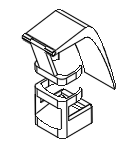
\includegraphics[width=3.25cm]{prototipo_arthropush.png}};

% Separador vertical
\draw[ArthroTeal!35, line width=0.8pt] (6.45,0.8) -- (6.45,8.2);

% ======================================================
% PANEL DERECHO GENERAL
% ======================================================
\fill[ArthroTeal!12, rounded corners=9pt] (6.85,0.75) rectangle (17.1,8.25);

% ======================================================
% TÍTULO PRINCIPAL
% ======================================================
\fill[white, rounded corners=7pt] (7.25,7.05) rectangle (16.7,8.0);

\node[
    text=ArthroNavy,
    font=\bfseries\large,
    align=center,
    text width=8.9cm
] at (11.98,7.52)
{ArthroPush};

% ======================================================
% BLOQUE INFORMACIÓN TÉCNICA
% ======================================================
\fill[white, rounded corners=7pt] (7.25,4.0) rectangle (12.35,6.75);

\node[
    anchor=north west,
    text=ArthroNavy,
    font=\bfseries\scriptsize,
    align=center,
    text width=4.55cm
] at (7.52,6.62)
{INFORMACIÓN TÉCNICA};

\node[
    anchor=north west,
    text=black,
    font=\fontsize{6.1}{7.0}\selectfont,
    align=left,
    text width=4.55cm
] at (7.50,6.15)
{\textbf{Modelo:} ARD-MDI-01\\
\textbf{Proyecto:} PR-PIB-GIS26-09\\
\textbf{Uso:} Adaptador para inhaladores MDI\\
\textbf{Material:} Polímero médico reciclable\\
\textbf{Función:} Ayuda a la pulsación manual\\
\textbf{Sin medicamento. No modifica dosis.}};

% ======================================================
% CÓDIGO DE BARRAS
% ======================================================
\fill[white, rounded corners=4pt] (7.55,2.72) rectangle (12.05,3.62);
\draw[black!20, rounded corners=4pt] (7.55,2.72) rectangle (12.05,3.62);

\foreach \x/\w in {
7.68/0.45,7.78/0.18,7.86/0.75,8.02/0.30,8.12/0.60,8.25/0.20,
8.36/0.95,8.52/0.35,8.64/0.70,8.78/0.20,8.90/0.85,9.05/0.30,
9.18/0.55,9.30/0.20,9.42/0.80,9.58/0.40,9.70/0.90,9.88/0.20,
10.00/0.50,10.12/0.25,10.25/0.95,10.44/0.35,10.57/0.70,
10.72/0.30,10.86/0.85,11.03/0.20,11.15/0.60,11.28/0.30,
11.40/0.95,11.58/0.40,11.72/0.75,11.88/0.20
}{
\draw[line width=\w mm] (\x,2.85) -- (\x,3.49);
}

\node[font=\fontsize{5.5}{6}\selectfont, text=black] at (9.8,2.63) {8 435672 091245};

% ======================================================
% BLOQUE ADVERTENCIAS
% ======================================================
\fill[white, rounded corners=7pt] (12.65,3.45) rectangle (16.7,6.75);

% Iconos advertencia más pequeños y separados del título
\draw[black!70, line width=0.35pt] (12.88,6.35) -- (13.03,6.58) -- (13.18,6.35) -- cycle;
\node[font=\tiny, text=black] at (13.03,6.41) {!};

\draw[black!70, line width=0.35pt] (16.17,6.35) -- (16.32,6.58) -- (16.47,6.35) -- cycle;
\node[font=\tiny, text=black] at (16.32,6.41) {!};

\node[
    text=ArthroNavy,
    font=\bfseries\scriptsize,
    align=center,
    text width=2.55cm
] at (14.56,5.9)
{ADVERTENCIAS\\DE USO};

\node[
    anchor=north west,
    text=black,
    font=\fontsize{5.15}{5.85}\selectfont,
    align=left,
    text width=3.45cm
] at (12.92,5.50)
{$\bullet$ Leer antes del uso.\\
$\bullet$ No usar si está dañado.\\
$\bullet$ Verificar ajuste estable.\\
$\bullet$ No forzar la palanca.\\
$\bullet$ Mantener fuera del alcance de niños.};

% ======================================================
% BLOQUE LIMPIEZA
% ======================================================
\fill[white, rounded corners=7pt] (7.25,1.22) rectangle (12.35,2.48);

\node[
    anchor=north west,
    text=ArthroNavy,
    font=\bfseries\scriptsize
] at (7.55,2.43)
{LIMPIEZA};

\node[
    anchor=north west,
    text=black,
    font=\fontsize{5.25}{5.9}\selectfont,
    align=left,
    text width=4.55cm
] at (7.55,2.08)
{Limpiar con paño húmedo y jabón neutro.\\
No usar disolventes ni abrasivos.\\
Conservar limpio, seco y protegido.};

% ======================================================
% BLOQUE INFORMACIÓN AMBIENTAL
% ======================================================
\fill[white, rounded corners=7pt] (12.65,1.35) rectangle (16.7,3.10);

\node[
    text=ArthroNavy,
    font=\bfseries\scriptsize,
    align=center,
    text width=3.5cm
] at (14.68,2.72)
{INFORMACIÓN\\AMBIENTAL};

\node[
    anchor=north west,
    text=black,
    font=\fontsize{5.35}{6.05}\selectfont,
    align=left,
    text width=3.45cm
] at (12.9,2.35)
{$\bullet$ Material reciclable.\\
$\bullet$ Separar del inhalador.\\
$\bullet$ Reciclar según normativa local.};

% Icono reciclaje sencillo
\node[text=ArthroTeal, font=\bfseries\small] at (16.28,2.82) {$\circlearrowleft$};

% ======================================================
% BLOQUE INFERIOR: TRAZABILIDAD + EMPRESA
% ======================================================
\fill[ArthroNavy!10, rounded corners=6pt] (7.25,0.42) rectangle (16.7,1.18);

\node[
    anchor=west,
    text=ArthroNavy,
    font=\fontsize{4.2}{4.9}\selectfont,
    align=left,
    text width=5.2cm
] at (7.35,0.82)
{
\textbf{Fabricado por:} ArthroDesign Solutions S.L.\\
Málaga, España
};

\node[
    anchor=west,
    text=ArthroNavy,
    font=\fontsize{4.2}{4.9}\selectfont,
    align=left,
    text width=4.3cm
] at (12.20,0.82)
{
\textbf{Contacto:} contacto@arthrodesign.com\\
\textbf{LOT-XXXX} · \textbf{MM/AAAA} · \textbf{v1.0}
};

\end{tikzpicture}%
}
\caption{Diseño propuesto de la etiqueta exterior del embalaje.}
\end{figure}




% ======================================================
% MANUAL DE INSTRUCCIONES DEL PRODUCTO
% ======================================================


\clearpage
\section{MANUAL DE INSTRUCCIONES}
\begin{center}

% ------------------------------------------------------
% CABECERA DEL MANUAL
% ------------------------------------------------------
\vspace*{0.2cm}

{\Huge\bfseries\color{ArthroNavy} MANUAL DE USUARIO}

\vspace{0.15cm}

{\Large\bfseries\color{ArthroTeal} ArthroPush}

\vspace{0.15cm}

{\normalsize Adaptador ergonómico para inhaladores de dosis medida (MDI)}

\vspace{0.35cm}

\noindent
\color{ArthroTeal}\rule{0.9\textwidth}{1.2pt}


% ------------------------------------------------------
% ILUSTRACIÓN PRINCIPAL DEL MANUAL
% ------------------------------------------------------
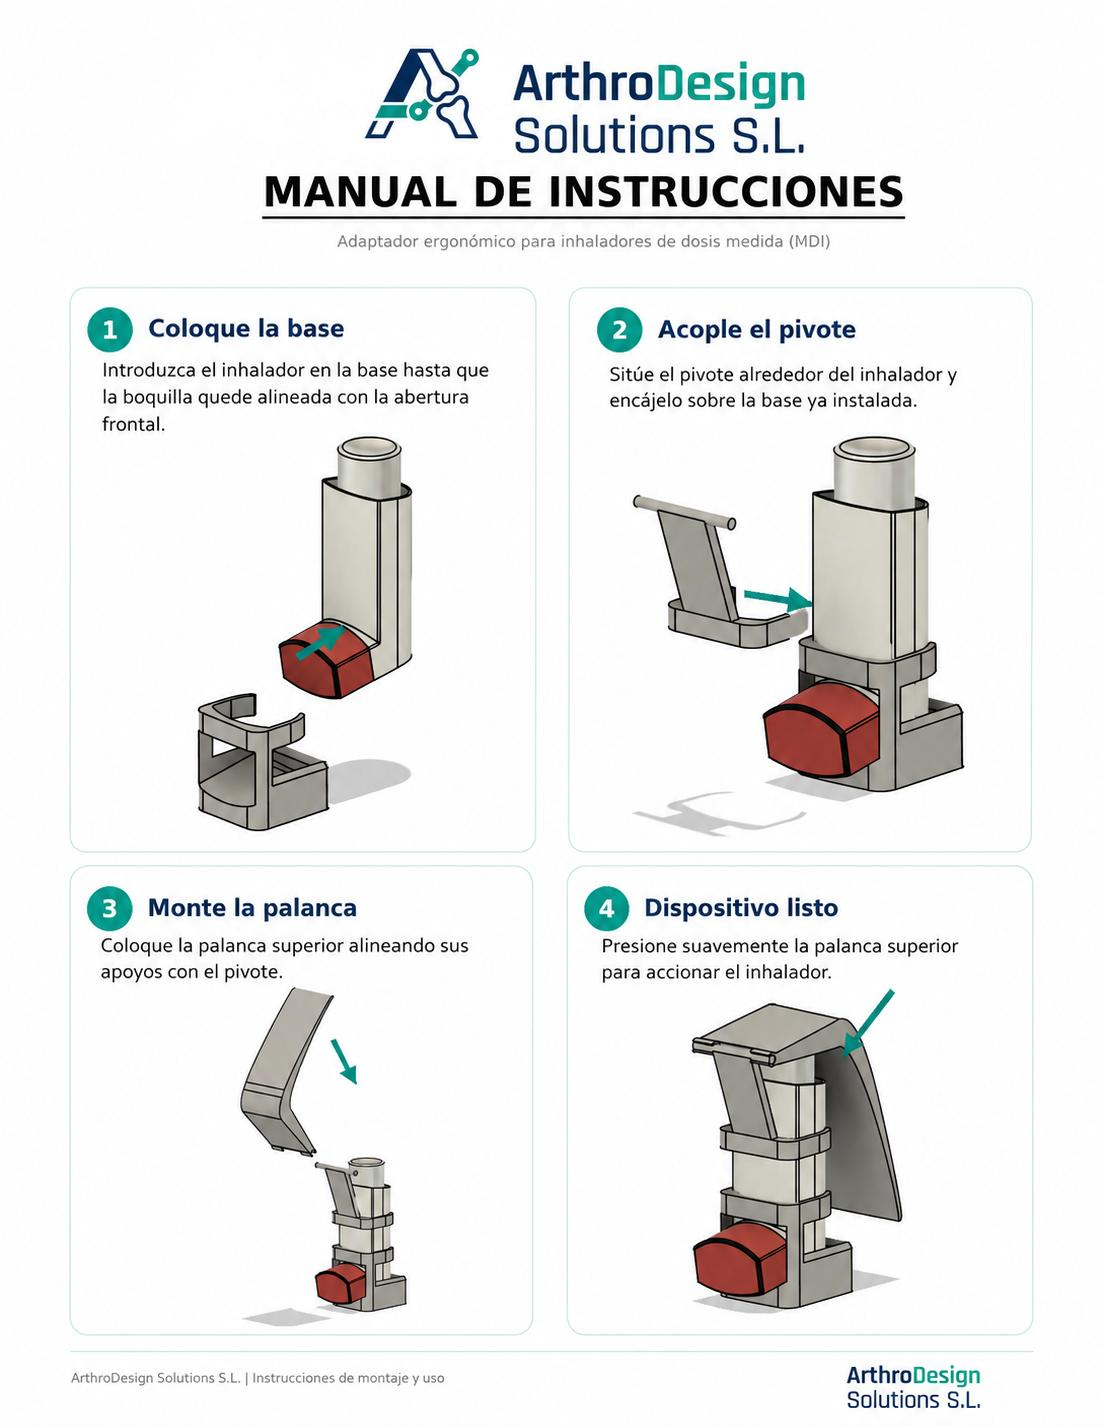
\includegraphics[width=0.88\textwidth]{manual_instrucciones_arthrodesign_logo_centrado.pdf}

\vspace{0.3cm}

{\small \textcolor{black} {Figura 2: Ilustración de montaje y uso del adaptador ArthroPush.}}

\vspace{0.5cm}

\end{center}

% ------------------------------------------------------
% BLOQUE GENERAL DEL MANUAL
% ------------------------------------------------------
\noindent
\begin{minipage}{\textwidth}
\setlength{\fboxsep}{10pt}
\colorbox{ArthroTeal!8}{
\begin{minipage}{0.96\textwidth}

{\large\bfseries\color{ArthroNavy} 1. Contenido del producto}

\vspace{0.2cm}

El conjunto ArthroPush está formado por tres componentes principales:

\begin{itemize}
    \item \textbf{Base:} pieza inferior que sujeta el inhalador y deja libre la boquilla de salida.
    \item \textbf{Pivote:} pieza de unión que abraza el inhalador y permite fijar el mecanismo.
    \item \textbf{Palanca:} pieza superior ergonómica que transmite la presión al cartucho del inhalador.
\end{itemize}

\end{minipage}
}
\end{minipage}

\vspace{0.4cm}

% ------------------------------------------------------
% MONTAJE
% ------------------------------------------------------
\noindent
\begin{minipage}{\textwidth}
\setlength{\fboxsep}{10pt}
\colorbox{white}{
\begin{minipage}{0.96\textwidth}

{\large\bfseries\color{ArthroNavy} 2. Montaje}

\vspace{0.2cm}

\begin{enumerate}
    \item \textbf{Colocar la base.} Introduzca el inhalador en la base, asegurando que la boquilla sobresale por el orificio frontal y queda libre.
    \item \textbf{Acoplar el pivote.} Sitúe el pivote alrededor del inhalador y encájelo sobre la base ya instalada.
    \item \textbf{Montar la palanca.} Coloque la palanca superior alineando sus apoyos con el pivote.
    \item \textbf{Comprobar el conjunto.} Verifique que el inhalador queda estable y que la palanca se mueve sin atascarse.
\end{enumerate}

\end{minipage}
}
\end{minipage}

\vspace{0.4cm}

% ------------------------------------------------------
% USO
% ------------------------------------------------------
\noindent
\begin{minipage}{0.48\textwidth}
\setlength{\fboxsep}{9pt}
\colorbox{ArthroTeal!8}{
\begin{minipage}{0.92\textwidth}

{\large\bfseries\color{ArthroNavy} 3. Uso}

\vspace{0.2cm}

\begin{enumerate}
    \item Agite el inhalador si lo indican sus instrucciones.
    \item Sujete el conjunto de forma estable.
    \item Coloque la boquilla según la pauta del medicamento.
    \item Presione suavemente la palanca hacia abajo para accionar el inhalador.
\end{enumerate}

\end{minipage}
}
\end{minipage}
\hfill
\begin{minipage}{0.48\textwidth}
\setlength{\fboxsep}{9pt}
\colorbox{ArthroTeal!8}{
\begin{minipage}{0.92\textwidth}

{\large\bfseries\color{ArthroNavy} 4. Retirada}

\vspace{0.2cm}

\begin{enumerate}
    \item Asegúrese de que el inhalador no está siendo presionado.
    \item Retire primero la palanca si es necesario.
    \item Extraiga el pivote y saque el inhalador de la base sin forzar las piezas.
\end{enumerate}

\end{minipage}
}
\end{minipage}

\vspace{0.45cm}

% ------------------------------------------------------
% ADVERTENCIAS
% ------------------------------------------------------
\noindent
\begin{minipage}{\textwidth}
\setlength{\fboxsep}{10pt}
\colorbox{ArthroNavy!8}{
\begin{minipage}{0.96\textwidth}

{\large\bfseries\color{ArthroNavy} 5. Advertencias}

\vspace{0.2cm}

\begin{itemize}
    \item ArthroPush no contiene medicamento y no modifica la dosis administrada.
    \item Siga siempre las instrucciones del inhalador y la pauta indicada por el profesional sanitario.
    \item No utilice el adaptador si presenta roturas, deformaciones, bordes dañados o ajuste inestable.
    \item No use el producto si el inhalador queda suelto, inclinado o mal alineado.
    \item No fuerce la palanca si ofrece resistencia anormal.
    \item Mantener fuera del alcance de niños sin supervisión.
\end{itemize}

\end{minipage}
}
\end{minipage}

\vspace{0.45cm}

% ------------------------------------------------------
% LIMPIEZA Y CONSERVACIÓN
% ------------------------------------------------------
\noindent
\begin{minipage}{0.48\textwidth}
\setlength{\fboxsep}{9pt}
\colorbox{white}{
\begin{minipage}{0.92\textwidth}

{\large\bfseries\color{ArthroNavy} 6. Limpieza}

\vspace{0.2cm}

Limpiar con un paño húmedo, agua tibia y jabón neutro. Secar completamente antes de volver a usar.

\vspace{0.15cm}

No utilizar disolventes, lejía, alcohol concentrado ni productos abrasivos.

\end{minipage}
}
\end{minipage}
\hfill
\begin{minipage}{0.48\textwidth}
\setlength{\fboxsep}{9pt}
\colorbox{white}{
\begin{minipage}{0.92\textwidth}

{\large\bfseries\color{ArthroNavy} 7. Conservación}

\vspace{0.2cm}

Guardar en un lugar limpio, seco y protegido de golpes.

\vspace{0.15cm}

No exponer a calor extremo, humedad excesiva ni productos químicos agresivos.

\end{minipage}
}
\end{minipage}

\vspace{0.5cm}

% ------------------------------------------------------
% PIE DEL MANUAL
% ------------------------------------------------------
\begin{center}
\color{ArthroTeal}\rule{0.9\textwidth}{1pt}

\vspace{0.15cm}

{\small\textbf{Fabricado por:} ArthroDesign Solutions S.L. \quad | \quad \textbf{Producto:} ArthroPush \quad | \quad \textbf{Modelo:} ARD-MDI-01}

\vspace{0.1cm}

{\small Málaga, España \quad | \quad contacto@arthrodesign.com}
\end{center}

\newpage

% ======================================================
% BLOQUE DE FIRMAS
% ======================================================
\noindent\begin{minipage}{\textwidth}
    \begin{flushright}
        En Málaga, a \today
    \end{flushright}
    \vspace{2cm}

    \noindent
    \begin{minipage}[t]{0.45\textwidth}
        \centering
        \rule{6cm}{0.6pt} \\
        \textbf{Fdo. D. Sergio Carmona Muñoz} \\
        Colegiado Nº 06424 \\
        DNI: 26291930D
    \end{minipage}
    \hfill
    \begin{minipage}[t]{0.45\textwidth}
        \centering
        \rule{6cm}{0.6pt} \\
        \textbf{Fdo. D. Juan Gabriel Navarro Valdivielso} \\
        Colegiado Nº 06425 \\
        DNI: 77666662D
    \end{minipage}

    \vspace{2cm}

    \noindent
    \begin{minipage}[t]{0.45\textwidth}
        \centering
        \rule{6cm}{0.6pt} \\
        \textbf{Fdo. D. Antonio Sánchez Doña} \\
        Colegiado Nº 06423 \\
        DNI: 79380534J
    \end{minipage}
    \hfill
    \begin{minipage}[t]{0.45\textwidth}
        \centering
        \rule{6cm}{0.6pt} \\
        \textbf{Fdo. D. Iván de la Torre Segato} \\
        Colegiado Nº 06421 \\
        DNI: 79383630G
    \end{minipage}
\end{minipage}
\vspace{1cm}

% ======================================================
% HOJA EN BLANCO CON MARCA DE AGUA
% ======================================================
\newpage
\pagestyle{fancy}

\begin{tikzpicture}[remember picture, overlay]
    \node[opacity=0.1] at (current page.center) {
\includegraphics[width=12cm]{logo_definitivo.png}};
\end{tikzpicture}

% Empujamos el texto hacia la parte inferior del folio
\vspace*{8.5cm} 
\begin{center}
    \textit{Esta hoja ha sido dejada deliberadamente en blanco.}
\end{center}
\vfill

\end{document}